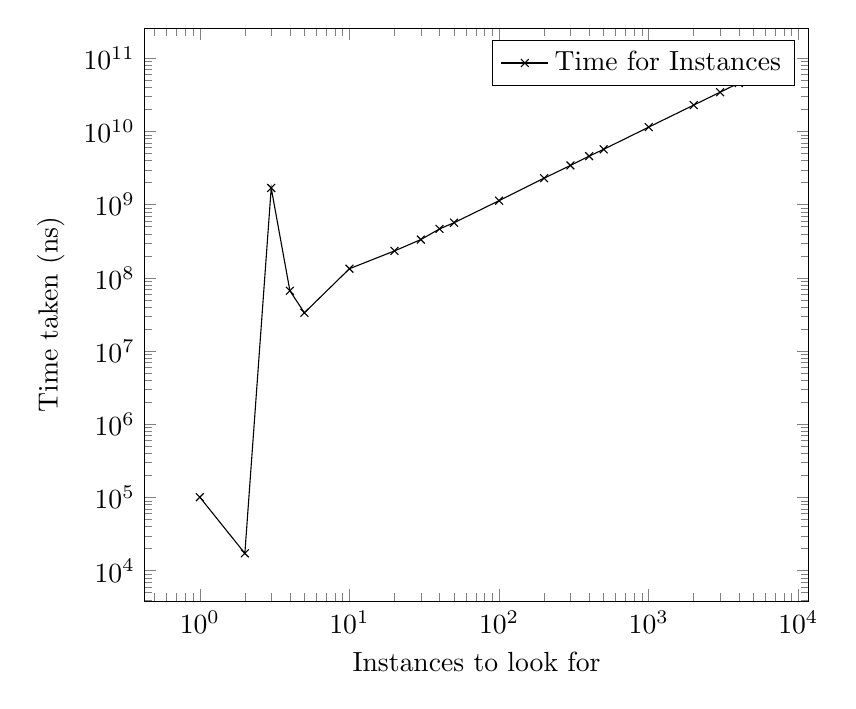
\begin{tikzpicture}

    \pgfplotsset{
        scale only axis,
    }

    \begin{axis}[
        xlabel=Instances to look for,
        ylabel=Time taken (ns),
        xmode=log,
        ymode=log
    ]
    \addplot[mark=x]
        coordinates{ % plot 1 data set
            ( 1 , 101053 )
            ( 2 , 17291 )
            ( 3 , 1.6937e+09 )
            ( 4 , 6.67496e+07 )
            ( 5 , 3.34086e+07 )
            ( 10 , 1.33625e+08 )
            ( 20 , 2.33841e+08 )
            ( 30 , 3.34033e+08 )
            ( 40 , 4.67719e+08 )
            ( 50 , 5.67789e+08 )
            ( 100 , 1.13591e+09 )
            ( 200 , 2.30494e+09 )
            ( 300 , 3.44066e+09 )
            ( 400 , 4.6101e+09 )
            ( 500 , 5.71234e+09 )
            ( 1000 , 1.14914e+10 )
            ( 2000 , 2.29831e+10 )
            ( 3000 , 3.44411e+10 )
            ( 4000 , 4.59325e+10 )
            ( 5000 , 5.74241e+10 )
        }; \label{plot_one}

        % plot 1 legend entry
        \addlegendimage{/pgfplots/refstyle=plot_one}
        \addlegendentry{Time for Instances}
    \end{axis}

\end{tikzpicture}